\section{Answer formation is staged}

The first lesson is measurement. A correct-vs-rest endpoint margin tells us whether the final answer is correct and separated, but it does not tell us when the final answer became competitive, how often the leader changed, or whether the final separation was already present. We therefore track the leader, runner-up, entropy, persistent ranks, and final-pair margin through depth.

Figure~\ref{fig:staged-summary} shows the central broad-panel result. The curve for $d_2$ lies to the left of $d_1$, and both lie to the left of $d_{50}$. In pooled rows, the median normalized depths are \PooledMedianDTwo{} for persistent contender status, \PooledMedianDOne{} for persistent winner status, and \PooledMedianDFifty{} for persistent decisive margin.

\begin{figure*}[t]
\centering
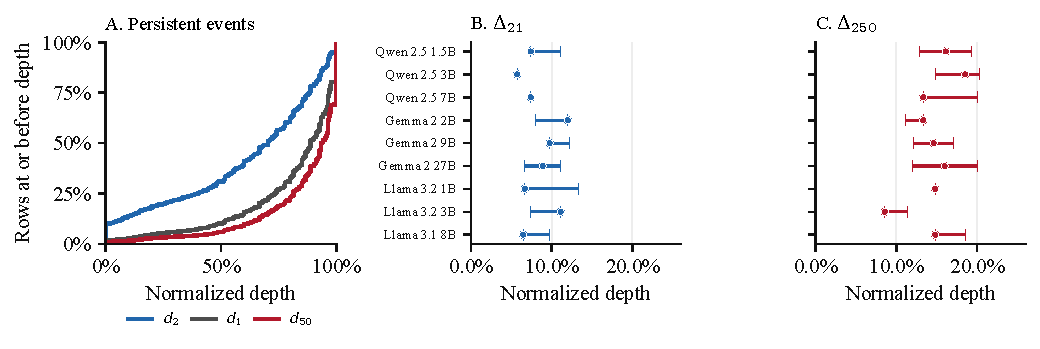
\includegraphics[width=\linewidth]{figure1_staged_summary.pdf}
\caption{\textbf{Answer formation is staged across depth.} Left: persistent contender status, persistent winner status, and persistent decisive margin arrive at different depths. Middle/right: model-level median lags with 95\% bootstrap intervals.}
\label{fig:staged-summary}
\end{figure*}

The separation among the three curves means that contender status, winner status, and decisive separation are not interchangeable readouts. A row can already carry the eventual answer among the leading options while the final-pair margin is still being written. Endpoint accuracy and final margins collapse these events into one terminal observation.

The main lag is $\Delta_{250}$, from persistent contender status to persistent decisive margin. Its pooled median is \PooledMedianDeltaTwentyFifty{}, with a 95\% bootstrap interval of [\PooledDeltaTwentyFiftyLow{}, \PooledDeltaTwentyFiftyHigh{}]. The smaller lag $\Delta_{21}$, from persistent contender to persistent top-1, has pooled median \PooledMedianDeltaTwentyOne{} with interval [\PooledDeltaTwentyOneLow{}, \PooledDeltaTwentyOneHigh{}].

Across models, the lags in Figure~\ref{fig:staged-summary} occupy a visible part of model depth rather than a single boundary layer. This staged view is the organizing principle for the rest of the paper. Candidate formation, winner selection, and decisive separation are related but distinct events in the score trajectory.
